\documentclass[12pt]{article}
\usepackage{amsmath}
\usepackage{graphicx,psfrag,epsf}
\usepackage{enumerate}
\usepackage{natbib}
\usepackage{url} % not crucial - just used below for the URL 

%\pdfminorversion=4
% NOTE: To produce blinded version, replace "0" with "1" below.
\newcommand{\blind}{0}

% DON'T change margins - should be 1 inch all around.
\addtolength{\oddsidemargin}{-.5in}%
\addtolength{\evensidemargin}{-.5in}%
\addtolength{\textwidth}{1in}%
\addtolength{\textheight}{1.3in}%
\addtolength{\topmargin}{-.8in}%

\newcommand{\logit}{\mathrm{lgt}}
\newcommand{\I}{\mathrm{I}}
\newcommand{\E}{\mathrm{E}}
\newcommand{\p}{\mathrm{P}}
\newcommand{\e}{\mathrm{e}}
\renewcommand{\o}{\omega}
\newcommand{\vecm}{\mathrm{vec}}
\newcommand{\kp}{\otimes}
\newcommand{\diag}{\mathrm{diag}}
\newcommand{\cov}{\mathrm{cov}}
\newcommand{\eps}{\epsilon}
\newcommand{\ep}{\varepsilon}
\newcommand{\obdots}{\ddots}    % change this later
\newcommand{\Ex}{{\cal E}}
\newcommand{\Exd}{\Ex_d}
\newcommand{\Es}{\E_\phi}
\newcommand{\rat}{{\frac{c_{ij}}{c_{i,j-1}}}}
\newcommand{\rmu}{m}
\newcommand{\rsig}{\nu}
\newcommand{\fd}{\mu}
\newcommand{\tr}{\mathrm{tr}}
\newcommand{\cor}{\mathrm{cor}}
\newcommand{\bx}[1]{\ensuremath{\overline{#1}|}}
\newcommand{\an}[1]{\ensuremath{a_{\bx{#1}}}}

\newcommand{\bi}{\begin{itemize}}
\newcommand{\ei}{\end{itemize}}

\renewcommand{\i}{\item}
\newcommand{\sr}{\ensuremath{\mathrm{SRISK}}}
\newcommand{\cs}{\ensuremath{\mathrm{CS}}}
\newcommand{\cri}{\ensuremath{\mathrm{Crisis}}}
\newcommand{\var}{\ensuremath{\mathrm{VaR}}}
\newcommand{\covar}{\ensuremath{\mathrm{CoVaR}}}
\newcommand{\med}{\ensuremath{\mathrm{m}}}
\newcommand{\de}{\mathrm{d}}
\renewcommand{\v}{\ensuremath{\mathrm{v}_q}}
\newcommand{\m}{\ensuremath{\mathrm{m}}}
\newcommand{\tvar}{\ensuremath{\mathrm{TVaR}}}
\renewcommand{\c}{\ensuremath{\mathrm{CoVaR_q}}}
\renewcommand{\v}{\ensuremath{\mathrm{VaR}_q}}



\newcommand{\eref}[1]{(\ref{#1})}
\newcommand{\fref}[1]{Figure \ref{#1}}
\newcommand{\sref}[1]{\S\ref{#1}}
\newcommand{\tref}[1]{Table \ref{#1}}
\newcommand{\aref}[1]{Appendix \ref{#1}}

\newcommand{\cq}{\ , \qquad}




\begin{document}

%\bibliographystyle{natbib}

\def\spacingset#1{\renewcommand{\baselinestretch}%
{#1}\small\normalsize} \spacingset{1}


%%%%%%%%%%%%%%%%%%%%%%%%%%%%%%%%%%%%%%%%%%%%%%%%%%%%%%%%%%%%%%%%%%%%%%%%%%%%%%

\if0\blind
{
  \title{\bf Measuring background and systemic risk in finance}
  \author{Piet de Jong\thanks{
    The authors gratefully acknowledge CIFR, the Centre of International Financial Regulation for financial support and other assistance.}\hspace{.2cm}\\
    Department of Applied Finance and Actuarial Studies, Macquarie University\\
    and \\
    Department of Applied Finance and Actuarial Studies, Macquarie University}
  \maketitle
} \fi

\if1\blind
{
  \bigskip
  \bigskip
  \bigskip
  \begin{center}
    {\LARGE\bf Title}
\end{center}
  \medskip
} \fi

\bigskip
\begin{abstract}
(200 or fewer words.)
This article refines, builds on, and extends  SRISK methodology recently proposed in the literature.  The refinement is to define SRISK in terms of a put on the Basel shortfall.   This  is built on by defining the background and systemic stress  of a firm as unconditional and departure from unconditional  expectation of the put, the latter when a hypothetical systemic stress is applied.  Systemic stress is defined in terms of a random variable and can take on variety of forms including alternative scenarios in usual stress testing as well stress driven by the interaction of variables.  Stressor random variables  are chosen by the practitioner.  Stressed expectations are linear, a sector systemic stress is naturally defined as linear in the firm specific systemic stress.      Application is made to Australian financial data.
\end{abstract}

\noindent%
{\it Keywords:}  3 to 6 keywords, that do not appear in the title
\vfill

\newpage
\spacingset{1.45} % DON'T change the spacing!

\section{Month to month monitoring  of financial stress}\label{monitoring}
 \tref{twodates} contains real time stress calculations on the first trading day of  January 2009 and November 2014.  As before there is no look ahead bias -- all calculations on each of the two dates only use data available on the first day of the applicable month.   The initial eight rows in \tref{twodates} lists the eight banks used in this study. 
 
 \begin{table}[ht]
\caption{One month ahead stress calculations for Australian banks$^\dag$}\label{twodates}
\centering
\small
\vspace{4mm}
\begin{tabular}{l|rrrrr|rrrrr}
\hline
&\multicolumn{5}{c|}{January 2009}&\multicolumn{5}{c}{November 2014}\\
  \hline
bank & B-log& debt &\multicolumn{2}{c}{stress}&  B-def   & B-log& debt   & \multicolumn{2}{c}{stress}& B-def \\
  \cline{4-5}\cline{9-10}
       &  lev& prop    & back & syst & prob & lev& prop  & back & syst & prob \\
  \cline{2-11} 
         & $\ell_{it} $ & $\pi_{it}$ & $\mu^*_{it}$  & $s^*_{it}$ & $q_{it}$  
         & $\ell_{it} $ & $\pi_{it}$ & $\mu^*_{it}$  & $s^*_{it}$ & $q_{it}$  
        \\
  \hline
cba & 18.57 & 24.30 & 22.99 & 29.60 & 91.43 & -70.34 & 22.70 & 0.00 & 0.00 & 0.00 \\ 
  anz & 15.93 & 18.37 & 14.87 & 18.89 & 92.82 & -38.64 & 22.10 & 0.00 & 0.00 & 0.00 \\ 
  nab & 31.97 & 25.50 & 39.98 & 19.41 & 99.97 & -12.45 & 25.61 & 50.52 & 67.13 & 1.23 \\ 
  wbc & -1.55 & 22.84 & 5.86 & 23.94 & 40.42 & -53.84 & 22.03 & 0.00 & 0.00 & 0.00 \\ 
  mqg & 41.22 & 5.75 & 11.02 & 5.46 & 99.92 & -46.10 & 4.33 & 0.17 & 0.12 & 0.03 \\ 
  boq & 63.30 & 1.32 & 3.55 & 0.99 & 99.95 & -17.05 & 1.33 & 0.80 & 1.34 & 0.33 \\ 
  ben & 18.91 & 1.81 & 1.72 & 1.71 & 90.53 & -7.63 & 1.84 & 25.43 & 30.71 & 8.47 \\ 
  aba & -8.12 & 0.10 & 0.00 & 0.00 & 9.97 & 9.22 & 0.07 & 23.07 & 0.71 & 89.63 \\ 
  \hline
  $\Ex_d$ & 18.78 &  & 17.17 & 8.63 & 82.72 & -41.91 &  & 0.03 & 0.12 & 0.54 \\ 
  $\Sigma$ & 17.81 & $^\dag$2.42 & 15.28 & 10.18 & 96.72 & -44.22 & $^\dag$3.27 & 0.00 & 0.00 & 0.00 \\ 
\hline
\end{tabular}

$^\dag$All numbers multiplied by 100 except total debt (in \$bln).
\end{table}
\normalsize

January 2009 was a time of great stress for all eight banks.     The first  and second columns in the two halves of the table body contain the 
 Basel log--leverage $\ell_{it}$ and debt $\pi_{it}\equiv d_{it}/d_t$ (as a proportion of total debt) for each of the banks.  Six of the eight banks were in Basel default with positive capital shortfalls as indicated in by the $\ell_{it}$ column:   the two banks not in Basel default were wbc and aba.    Background and systemic stress
$$
\mu^*_{it} \equiv \frac{\pi_{it}\mu_{it}}{\Ex_d(\mu_{it})}\cq s^*_{it} \equiv \frac{\pi_{it}s_{it}}{\Ex_d(\mu_{it})}\ , 
$$
for the eight banks as well as the probability of a Basel default in one month $q_{it}$ and the proportion $\pi_{it}$ of total debt are displayed in the next 3 columns.    The background stress column indicates most of the background stress arises from nab -- almost 40\% of the total.   The next most background stressed bank is cba with wbc also a substantial contributor.   The mqg bank contributes almost double to background stress compared to the proportion of total debt  it carries.  The other three small banks contribute relatively little to background stress with boq  almost 3 times expected on the basis of its debt.   Systemic stress is highest for the cba, higher than expected on the basis of its debt load and hence cba was most susceptible to stress from additional general market equity devaluation.    All other banks appear have systemic stress comparable to their size in terms of debt load with only nab being less systemically important.    This should be compared to nab's high background stress.

Continuing with January 2009, the final two rows indicate the total amount of stress in the system and it's diversifiability.    
The second last  row labelled $\Ex_d$  displays, in order, $\Ex_d(\ell_{it})$, blank, $\overline{\mu}_t\equiv \Ex_d(\mu_{it})$, $\overline{s}_t\equiv\Ex_d(s_{it})$ and  $\Ex_d(q_{it})$.   The final row labelled $\Sigma$ displays the aggregate stress quantities,treating all eight banks as one entity, $\ell_t$, total debt $d_t$ in billions of dollars,  $\mu_t$, $s_t$, and  $q_t$.
On an aggregate basis background stress is about twice systemic stress.   Thus there is more danger of increasing capital shortfall due to market volatility  as opposed to further stress from further substantial general market devaluation.  The final row indicates stresses are not diversifiable:    The marginally  smaller  ``diversified"  background stress is offset by an increase in systemic stress.    Also the diversified probability of Basel default is higher than the debt weighted average.   

Stress readings  alter dramatically when moving to November 2014 -- there is virtually no stress in any bank and the small amount of  stress in the system is diversifiable.    Most of the  background stress is carried by nab with lesser contributions by ben and aba.    All the stress in the minor bank aba is background stress as only nab and nab have substantial systemic stress contributions.   Again, however, it must be emphasised that there is minimal systemic stress in the system.    Only aba has substantial Basel default probability, but this bank is a very minor player in the Australian banking scene.   Notice total debt in the banking sector  jumps about 35\% between January 2009 and November 2014.


\section{Further guidelines}

\begin{figure}
\begin{center}
%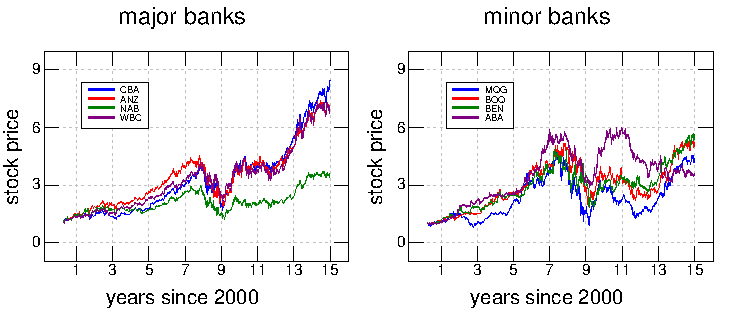
\includegraphics[width=3in]{fig1.pdf}
\end{center}
\caption{Consistency comparison in fitting surrogate model in the tidal
power example. \label{fig:first}}
\end{figure}

\begin{table}
\caption{D-optimality values for design $X$ under five different scenarios.  \label{tab:tabone}}
\begin{center}
\begin{tabular}{rrrrr}
one & two & three & four & five\\\hline
1.23 & 3.45 & 5.00 & 1.21 & 3.41 \\
1.23 & 3.45 & 5.00 & 1.21 & 3.42 \\
1.23 & 3.45 & 5.00 & 1.21 & 3.43 \\
\end{tabular}
\end{center}
\end{table}

\begin{itemize}
\item Note that figures and tables (such as Figure~\ref{fig:first} and
Table~\ref{tab:tabone}) should appear in the paper, not at the end or
in separate files.
\item In the latex source, near the top of the file the command
\verb+\newcommand{\blind}{1}+ can be used to hide the authors and
acknowledgements, producing the required blinded version.
\item Remember that in the blind version, you should not identify authors
indirectly in the text.  That is, don't say ``In Smith et. al.  (2009) we
showed that ...''.  Instead, say ``Smith et. al. (2009) showed that ...''.
\item These points are only intended to remind you of some requirements.
Please refer to the instructions for authors
at \url{http://amstat.tandfonline.com/action/authorSubmission?journalCode=ubes20&page=instructions#}
\item For more about ASA\ style, please see \url{http://journals.taylorandfrancis.com/amstat/asa-style-guide/}
\item If you have supplementary material (e.g., software, data, technical
proofs), identify them in the section below.  In early stages of the
submission process, you may be unsure what to include as supplementary
material.  Don't worry---this is something that can be worked out at later stages.
\end{itemize}

\section{Methods}
\label{sec:meth}
Don't take any of these section titles seriously.  They're just for
illustration.

\section{Verifications}
\label{sec:verify}
This section will be just long enough to illustrate what a full page of
text looks like, for margins and spacing.


\cite{Campbell02}, \cite{Schubert13}, \cite{Chi81}


The quick brown fox jumped over the lazy dog.
The quick brown fox jumped over the lazy dog.
The quick brown fox jumped over the lazy dog.
The quick brown fox jumped over the lazy dog.
{\bf With this spacing we have 30 lines per page.}
The quick brown fox jumped over the lazy dog.
The quick brown fox jumped over the lazy dog.
The quick brown fox jumped over the lazy dog.
The quick brown fox jumped over the lazy dog.
The quick brown fox jumped over the lazy dog.

The quick brown fox jumped over the lazy dog.
The quick brown fox jumped over the lazy dog.
The quick brown fox jumped over the lazy dog.
The quick brown fox jumped over the lazy dog.
The quick brown fox jumped over the lazy dog.
The quick brown fox jumped over the lazy dog.
The quick brown fox jumped over the lazy dog.
The quick brown fox jumped over the lazy dog.
The quick brown fox jumped over the lazy dog.
The quick brown fox jumped over the lazy dog.

The quick brown fox jumped over the lazy dog.
The quick brown fox jumped over the lazy dog.
The quick brown fox jumped over the lazy dog.
The quick brown fox jumped over the lazy dog.
The quick brown fox jumped over the lazy dog.
The quick brown fox jumped over the lazy dog.
The quick brown fox jumped over the lazy dog.
The quick brown fox jumped over the lazy dog.
The quick brown fox jumped over the lazy dog.
The quick brown fox jumped over the lazy dog.

The quick brown fox jumped over the lazy dog.
The quick brown fox jumped over the lazy dog.
The quick brown fox jumped over the lazy dog.
The quick brown fox jumped over the lazy dog.
The quick brown fox jumped over the lazy dog.
The quick brown fox jumped over the lazy dog.
The quick brown fox jumped over the lazy dog.
The quick brown fox jumped over the lazy dog.
The quick brown fox jumped over the lazy dog.
The quick brown fox jumped over the lazy dog.

The quick brown fox jumped over the lazy dog.
The quick brown fox jumped over the lazy dog.
The quick brown fox jumped over the lazy dog.
The quick brown fox jumped over the lazy dog.
The quick brown fox jumped over the lazy dog.
The quick brown fox jumped over the lazy dog.
The quick brown fox jumped over the lazy dog.
The quick brown fox jumped over the lazy dog.
The quick brown fox jumped over the lazy dog.
The quick brown fox jumped over the lazy dog.

The quick brown fox jumped over the lazy dog.
The quick brown fox jumped over the lazy dog.
The quick brown fox jumped over the lazy dog.
The quick brown fox jumped over the lazy dog.
The quick brown fox jumped over the lazy dog.
The quick brown fox jumped over the lazy dog.
The quick brown fox jumped over the lazy dog.
The quick brown fox jumped over the lazy dog.
The quick brown fox jumped over the lazy dog.
The quick brown fox jumped over the lazy dog.

The quick brown fox jumped over the lazy dog.
The quick brown fox jumped over the lazy dog.
The quick brown fox jumped over the lazy dog.
The quick brown fox jumped over the lazy dog.
The quick brown fox jumped over the lazy dog.
The quick brown fox jumped over the lazy dog.
The quick brown fox jumped over the lazy dog.
The quick brown fox jumped over the lazy dog.
The quick brown fox jumped over the lazy dog.
The quick brown fox jumped over the lazy dog.

The quick brown fox jumped over the lazy dog.
The quick brown fox jumped over the lazy dog.
The quick brown fox jumped over the lazy dog.
The quick brown fox jumped over the lazy dog.
The quick brown fox jumped over the lazy dog.
The quick brown fox jumped over the lazy dog.
The quick brown fox jumped over the lazy dog.
The quick brown fox jumped over the lazy dog.
The quick brown fox jumped over the lazy dog.
The quick brown fox jumped over the lazy dog.

The quick brown fox jumped over the lazy dog.
The quick brown fox jumped over the lazy dog.
The quick brown fox jumped over the lazy dog.
The quick brown fox jumped over the lazy dog.
The quick brown fox jumped over the lazy dog.
The quick brown fox jumped over the lazy dog.
The quick brown fox jumped over the lazy dog.
The quick brown fox jumped over the lazy dog.
The quick brown fox jumped over the lazy dog.
The quick brown fox jumped over the lazy dog.

The quick brown fox jumped over the lazy dog.
The quick brown fox jumped over the lazy dog.
The quick brown fox jumped over the lazy dog.
The quick brown fox jumped over the lazy dog.
The quick brown fox jumped over the lazy dog.
The quick brown fox jumped over the lazy dog.
The quick brown fox jumped over the lazy dog.
The quick brown fox jumped over the lazy dog.
The quick brown fox jumped over the lazy dog.
The quick brown fox jumped over the lazy dog.

The quick brown fox jumped over the lazy dog.
The quick brown fox jumped over the lazy dog.
The quick brown fox jumped over the lazy dog.
The quick brown fox jumped over the lazy dog.



\section{Conclusion}
\label{sec:conc}


\bigskip
\begin{center}
{\large\bf SUPPLEMENTARY MATERIAL}
\end{center}

\begin{description}

\item[Title:] Brief description. (file type)

\item[R-package for  MYNEW routine:] R-package �MYNEW� containing code to perform the diagnostic methods described in the article. The package also contains all datasets used as examples in the article. (GNU zipped tar file)

\item[HIV data set:] Data set used in the illustration of MYNEW method in Section~ 3.2. (.txt file)

\end{description}

\section{BibTeX}

We hope you've chosen to use BibTeX!\ If you have, please feel free to use the package natbib with any bibliography style you're comfortable with. The .bst file Chicago was used here, and agsm.bst has been included here for your convenience. 

\bibliographystyle{Chicago}

\bibliography{Bibliography-MM-MC}
\end{document}
